%%%%%%%%%%%%%
% 
% Alexander Powell
% Finite Automata
% Homework Assignment #3
% 9.23.2015
% 
%%%%%%%%%%%%%

\documentclass[11pt]{article}

\usepackage{times,mathptm}
\usepackage{pifont}
\usepackage{exscale}
\usepackage{latexsym}
\usepackage{amsmath}
\usepackage{amssymb}
\usepackage{amsthm}
\usepackage{epsfig}
\usepackage{tikz}


\textwidth 6.5in
\textheight 9in
\oddsidemargin -0.0in
\topmargin -0.0in

\parindent 0pt     % How much the first word of a paragraph is indented. 
\parskip 0pt	   % How much extra space to leave between paragraphs.

\begin{document}

\begin{center}             % If you only centering 1 line use \centerline{}
\begin{LARGE}
{\bf Finite Automata Homework 3}
\end{LARGE}
\vskip 0.25cm      % vertical skip (0.25 cm)

Due: Thursday, Sep 24\\  % force new line
Alexander Powell
\end{center}

\begin{enumerate}

\item
Let $D = \{w | w$ contains an even number of a’s and an odd number of b’s and does not contain the substring ab$\}$. Give a DFA with five states that recognizes $D$ and a
regular expression that generates $D$.  

The DFA that accepts the language $D$ is displayed below.  

\iffalse
\begin{center}
\begin{tikzpicture}[scale=0.2]
\tikzstyle{every node}+=[inner sep=0pt]
\draw [black] (43.7,-17.4) circle (3);
\draw (43.7,-17.4) node {$q_0$};
\draw [black] (60.9,-27.5) circle (3);
\draw (60.9,-27.5) node {$q_1$};
\draw [black] (60.9,-27.5) circle (2.4);
\draw [black] (26.5,-27.5) circle (3);
\draw (26.5,-27.5) node {$q_2$};
\draw [black] (16.9,-40.3) circle (3);
\draw (16.9,-40.3) node {$q_3$};
\draw [black] (16.9,-40.3) circle (2.4);
\draw [black] (43.7,-10.4) -- (43.7,-14.4);
\fill [black] (43.7,-14.4) -- (44.2,-13.6) -- (43.2,-13.6);
\draw [black] (46.693,-17.272) arc (87.12154:32.03476:16.126);
\fill [black] (59.55,-24.82) -- (59.55,-23.88) -- (58.71,-24.41);
\draw (55.05,-18.97) node [above] {$b$};
\draw [black] (57.907,-27.355) arc (-97.37943:-143.46427:18.697);
\fill [black] (45.29,-19.94) -- (45.36,-20.88) -- (46.16,-20.29);
\draw (49.84,-25.44) node [below] {$b$};
\draw [black] (41.11,-18.92) -- (29.09,-25.98);
\fill [black] (29.09,-25.98) -- (30.03,-26.01) -- (29.52,-25.14);
\draw (34.16,-21.95) node [above] {$a$};
\draw [black] (16.528,-37.334) arc (-181.3809:-252.3589:10.078);
\fill [black] (16.53,-37.33) -- (17.05,-36.55) -- (16.05,-36.52);
\draw (17.96,-30.13) node [left] {$a$};
\draw [black] (26.755,-30.479) arc (-3.34343:-70.39636:10.446);
\fill [black] (26.75,-30.48) -- (26.21,-31.25) -- (27.21,-31.31);
\draw (25.26,-37.53) node [right] {$a$};
\end{tikzpicture}
\end{center}
\fi

\begin{center}
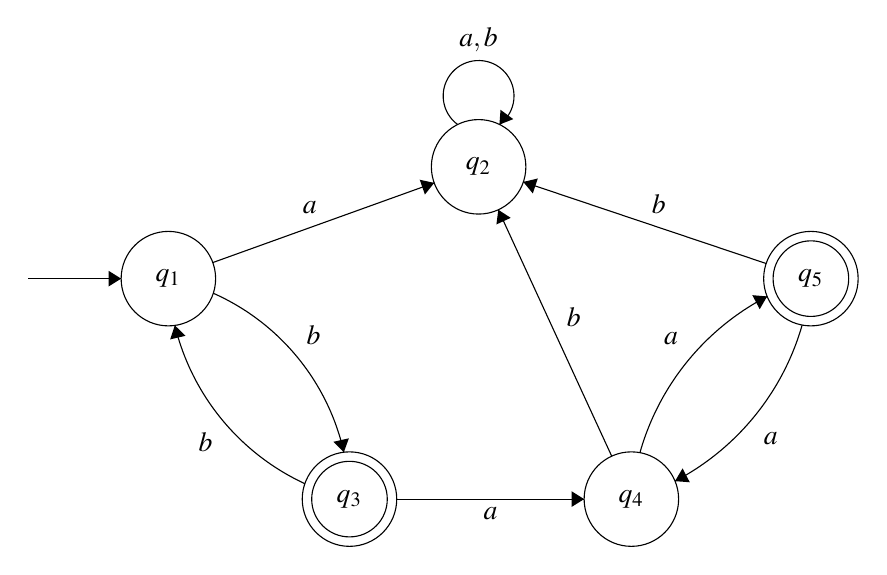
\begin{tikzpicture}[scale=0.2]
\tikzstyle{every node}+=[inner sep=0pt]
\draw [black] (17.2,-19.9) circle (3);
\draw (17.2,-19.9) node {$q_1$};
\draw [black] (28.7,-33.9) circle (3);
\draw (28.7,-33.9) node {$q_3$};
\draw [black] (28.7,-33.9) circle (2.4);
\draw [black] (36.9,-12.8) circle (3);
\draw (36.9,-12.8) node {$q_2$};
\draw [black] (46.6,-33.9) circle (3);
\draw (46.6,-33.9) node {$q_4$};
\draw [black] (58,-19.9) circle (3);
\draw (58,-19.9) node {$q_5$};
\draw [black] (58,-19.9) circle (2.4);
\draw [black] (20.02,-18.88) -- (34.08,-13.82);
\fill [black] (34.08,-13.82) -- (33.16,-13.62) -- (33.49,-14.56);
\draw (26.18,-15.82) node [above] {$a$};
\draw [black] (20.048,-20.826) arc (66.0867:12.71462:14.553);
\fill [black] (28.34,-30.93) -- (28.66,-30.04) -- (27.68,-30.26);
\draw (25.95,-23.46) node [right] {$b$};
\draw [black] (25.87,-32.921) arc (-114.82986:-166.36882:14.964);
\fill [black] (17.61,-22.87) -- (17.31,-23.76) -- (18.29,-23.53);
\draw (20.03,-30.27) node [left] {$b$};
\draw [black] (31.7,-33.9) -- (43.6,-33.9);
\fill [black] (43.6,-33.9) -- (42.8,-33.4) -- (42.8,-34.4);
\draw (37.65,-34.4) node [below] {$a$};
\draw [black] (47.143,-30.954) arc (164.2337:117.45543:16.122);
\fill [black] (55.22,-21.03) -- (54.28,-20.95) -- (54.75,-21.84);
\draw (49.6,-23.73) node [left] {$a$};
\draw [black] (57.445,-22.844) arc (-15.96118:-62.34969:16.235);
\fill [black] (49.37,-32.76) -- (50.31,-32.83) -- (49.85,-31.95);
\draw (54.98,-30.06) node [right] {$a$};
\draw [black] (45.35,-31.17) -- (38.15,-15.53);
\fill [black] (38.15,-15.53) -- (38.03,-16.46) -- (38.94,-16.04);
\draw (42.47,-22.32) node [right] {$b$};
\draw [black] (55.16,-18.94) -- (39.74,-13.76);
\fill [black] (39.74,-13.76) -- (40.34,-14.49) -- (40.66,-13.54);
\draw (48.34,-15.81) node [above] {$b$};
\draw [black] (35.577,-10.12) arc (234:-54:2.25);
\draw (36.9,-5.55) node [above] {$a,b$};
\fill [black] (38.22,-10.12) -- (39.1,-9.77) -- (38.29,-9.18);
\draw [black] (8.3,-19.9) -- (14.2,-19.9);
\fill [black] (14.2,-19.9) -- (13.4,-19.4) -- (13.4,-20.4);
\end{tikzpicture}
\end{center}

The regular expression that generates $D$ is written as 
$$ b(bb)^*(aa)^* $$

\item
Use the procedure described in Lemma $1.60$ to convert the following finite automata to regular expressions.

The given finite automata is shown below.  

\begin{center}
\begin{tikzpicture}[scale=0.2]
\tikzstyle{every node}+=[inner sep=0pt]
\draw [black] (20.6,-11.4) circle (3);
\draw (20.6,-11.4) node {$1$};
\draw [black] (20.6,-11.4) circle (2.4);
\draw [black] (50,-11.4) circle (3);
\draw (50,-11.4) node {$2$};
\draw [black] (35.5,-33.8) circle (3);
\draw (35.5,-33.8) node {$3$};
\draw [black] (35.5,-33.8) circle (2.4);
\draw [black] (33.84,-31.3) -- (22.26,-13.9);
\fill [black] (22.26,-13.9) -- (22.29,-14.84) -- (23.12,-14.29);
\draw (27.44,-23.93) node [left] {$a$};
\draw [black] (36.083,-30.858) arc (166.1383:128.03:32.333);
\fill [black] (47.55,-13.14) -- (46.62,-13.24) -- (47.23,-14.02);
\draw (39.71,-19.72) node [left] {$b$};
\draw [black] (49.375,-14.333) arc (-14.58662:-51.24508:33.516);
\fill [black] (37.92,-32.03) -- (38.86,-31.92) -- (38.23,-31.14);
\draw (45.69,-25.42) node [right] {$b$};
\draw [black] (23.6,-11.4) -- (47,-11.4);
\fill [black] (47,-11.4) -- (46.2,-10.9) -- (46.2,-11.9);
\draw (35.3,-10.9) node [above] {$a,\mbox{ }b$};
\draw [black] (51.232,-8.677) arc (183.38789:-104.61211:2.25);
\draw (55.77,-5.68) node [right] {$a$};
\fill [black] (52.91,-10.72) -- (53.74,-11.17) -- (53.68,-10.18);
\draw [black] (12.7,-11.4) -- (17.6,-11.4);
\fill [black] (17.6,-11.4) -- (16.8,-10.9) -- (16.8,-11.9);
\end{tikzpicture}
\end{center}

By converting to a GNFA, we get the following structure:

\begin{center}
\begin{tikzpicture}[scale=0.2]
\tikzstyle{every node}+=[inner sep=0pt]
\draw [black] (24,-18.4) circle (3);
\draw (24,-18.4) node {$1$};
\draw [black] (50,-11.4) circle (3);
\draw (50,-11.4) node {$2$};
\draw [black] (44.1,-36.3) circle (3);
\draw (44.1,-36.3) node {$3$};
\draw [black] (9.8,-18.4) circle (3);
\draw (9.8,-18.4) node {$S$};
\draw [black] (24,-41.4) circle (3);
\draw (24,-41.4) node {$A$};
\draw [black] (24,-41.4) circle (2.4);
\draw [black] (41.86,-34.3) -- (26.24,-20.4);
\fill [black] (26.24,-20.4) -- (26.51,-21.3) -- (27.17,-20.55);
\draw (33.09,-27.84) node [below] {$a$};
\draw [black] (43.622,-33.34) arc (-173.71222:-212.94831:29.856);
\fill [black] (48.24,-13.83) -- (47.39,-14.23) -- (48.23,-14.77);
\draw (43.49,-22.77) node [left] {$b$};
\draw [black] (50.434,-14.367) arc (5.54075:-32.20128:30.941);
\fill [black] (45.82,-33.84) -- (46.67,-33.43) -- (45.82,-32.9);
\draw (50.5,-24.91) node [right] {$b$};
\draw [black] (26.9,-17.62) -- (47.1,-12.18);
\fill [black] (47.1,-12.18) -- (46.2,-11.91) -- (46.46,-12.87);
\draw (35.5,-14.28) node [above] {$a,\mbox{ }b$};
\draw [black] (12.8,-18.4) -- (21,-18.4);
\fill [black] (21,-18.4) -- (20.2,-17.9) -- (20.2,-18.9);
\draw (16.9,-18.9) node [below] {$\epsilon$};
\draw [black] (24,-21.4) -- (24,-38.4);
\fill [black] (24,-38.4) -- (24.5,-37.6) -- (23.5,-37.6);
\draw (23.5,-29.9) node [left] {$\epsilon$};
\draw [black] (41.19,-37.04) -- (26.91,-40.66);
\fill [black] (26.91,-40.66) -- (27.81,-40.95) -- (27.56,-39.98);
\draw (33.36,-38.29) node [above] {$\epsilon$};
\draw [black] (50.81,-8.523) arc (192.01279:-95.98721:2.25);
\draw (55.47,-5.89) node [above] {$a$};
\fill [black] (52.78,-10.29) -- (53.66,-10.62) -- (53.45,-9.64);
\end{tikzpicture}
\end{center}

After removing state $1$, we get a structure that looks like the following:

\begin{center}
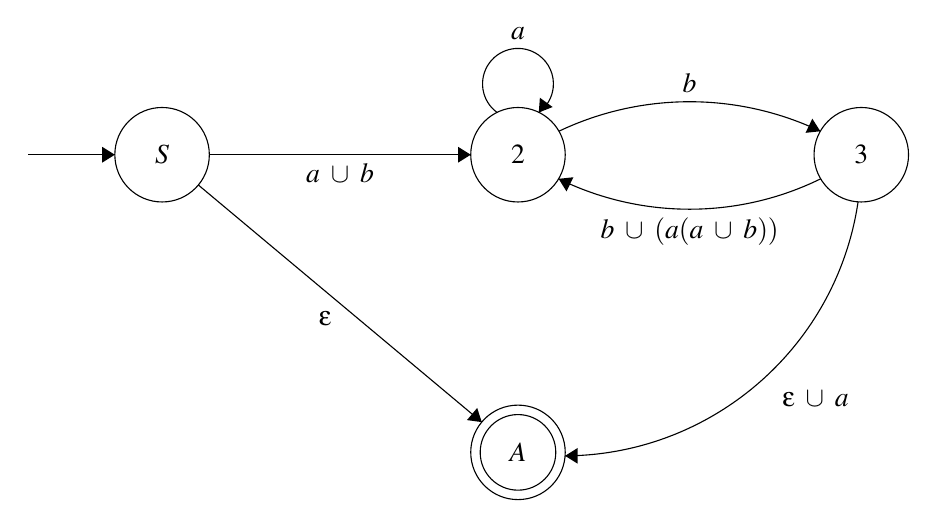
\begin{tikzpicture}[scale=0.2]
\tikzstyle{every node}+=[inner sep=0pt]
\draw [black] (13.4,-14.2) circle (3);
\draw (13.4,-14.2) node {$S$};
\draw [black] (36,-14.2) circle (3);
\draw (36,-14.2) node {$2$};
\draw [black] (57.8,-14.2) circle (3);
\draw (57.8,-14.2) node {$3$};
\draw [black] (36,-33.1) circle (3);
\draw (36,-33.1) node {$A$};
\draw [black] (36,-33.1) circle (2.4);
\draw [black] (15.7,-16.12) -- (33.7,-31.18);
\fill [black] (33.7,-31.18) -- (33.41,-30.28) -- (32.76,-31.05);
\draw (23.75,-24.14) node [below] {$\epsilon$};
\draw [black] (16.4,-14.2) -- (33,-14.2);
\fill [black] (33,-14.2) -- (32.2,-13.7) -- (32.2,-14.7);
\draw (24.7,-14.7) node [below] {$a\mbox{ }\cup\mbox{ }b$};
\draw [black] (38.599,-12.707) arc (115.43306:64.56694:19.33);
\fill [black] (55.2,-12.71) -- (54.69,-11.91) -- (54.26,-12.81);
\draw (46.9,-10.33) node [above] {$b$};
\draw [black] (55.222,-15.729) arc (-63.87574:-116.12426:18.901);
\fill [black] (38.58,-15.73) -- (39.08,-16.53) -- (39.52,-15.63);
\draw (46.9,-18.16) node [below] {$b\mbox{ }\cup\mbox{ }(a(a\mbox{ }\cup\mbox{ }b))$};
\draw [black] (34.677,-11.52) arc (234:-54:2.25);
\draw (36,-6.95) node [above] {$a$};
\fill [black] (37.32,-11.52) -- (38.2,-11.17) -- (37.39,-10.58);
\draw [black] (57.596,-17.19) arc (-8.4418:-89.70942:18.909);
\fill [black] (38.99,-33.32) -- (39.79,-33.82) -- (39.79,-32.82);
\draw (54.9,-29.19) node [below] {$\epsilon\mbox{ }\cup\mbox{ }a$};
\draw [black] (4.9,-14.2) -- (10.4,-14.2);
\fill [black] (10.4,-14.2) -- (9.6,-13.7) -- (9.6,-14.7);
\end{tikzpicture}
\end{center}

After removing state $2$, we get a structure that looks like the following:

\begin{center}
\begin{tikzpicture}[scale=0.2]
\tikzstyle{every node}+=[inner sep=0pt]
\draw [black] (18.1,-20.6) circle (3);
\draw (18.1,-20.6) node {$S$};
\draw [black] (55.5,-20.6) circle (3);
\draw (55.5,-20.6) node {$3$};
\draw [black] (36,-33.1) circle (3);
\draw (36,-33.1) node {$A$};
\draw [black] (36,-33.1) circle (2.4);
\draw [black] (20.56,-22.32) -- (33.54,-31.38);
\fill [black] (33.54,-31.38) -- (33.17,-30.51) -- (32.6,-31.33);
\draw (26.1,-27.35) node [below] {$\epsilon$};
\draw [black] (52.97,-22.22) -- (38.53,-31.48);
\fill [black] (38.53,-31.48) -- (39.47,-31.47) -- (38.93,-30.63);
\draw (49.36,-27.35) node [below] {$\epsilon\mbox{ }\cup\mbox{ }a$};
\draw [black] (9.6,-20.6) -- (15.1,-20.6);
\fill [black] (15.1,-20.6) -- (14.3,-20.1) -- (14.3,-21.1);
\draw [black] (54.678,-17.727) arc (223.69515:-64.30485:2.25);
\draw (62.02,-12.47) node [above] {$(b\mbox{ }\cup\mbox{ }(a(a\mbox{ }\cup\mbox{ }b)))a^*b$};
\fill [black] (57.28,-18.2) -- (58.2,-18.01) -- (57.51,-17.29);
\draw [black] (21.1,-20.6) -- (52.5,-20.6);
\fill [black] (52.5,-20.6) -- (51.7,-20.1) -- (51.7,-21.1);
\draw (36.8,-20.1) node [above] {$(a\mbox{ }\cup\mbox{ }b)a^*b$};
\end{tikzpicture}
\end{center}

Finally, after removing state $3$, we get the finite automaton below:

\begin{center}
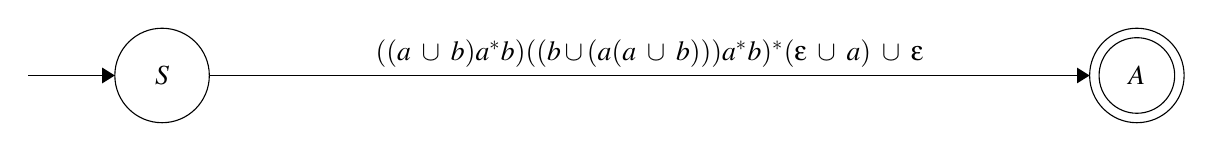
\begin{tikzpicture}[scale=0.2]
\tikzstyle{every node}+=[inner sep=0pt]
\draw [black] (10,-20.6) circle (3);
\draw (10,-20.6) node {$S$};
\draw [black] (71.9,-20.6) circle (3);
\draw (71.9,-20.6) node {$A$};
\draw [black] (71.9,-20.6) circle (2.4);
\draw [black] (13,-20.6) -- (68.9,-20.6);
\fill [black] (68.9,-20.6) -- (68.1,-20.1) -- (68.1,-21.1);
\draw (40.95,-20.1) node [above] {$((a\mbox{ }\cup\mbox{ }b)a^*b)((b\cup(a(a\mbox{ }\cup\mbox{ }b)))a^*b)^*(\epsilon\mbox{ }\cup\mbox{ }a)\mbox{ }\cup\mbox{ }\epsilon$};
\draw [black] (1.5,-20.6) -- (7,-20.6);
\fill [black] (7,-20.6) -- (6.2,-20.1) -- (6.2,-21.1);
\end{tikzpicture}
\end{center}

So the regular expression that generates the language can be written as 
$$ ((a \cup b)a^*b)((b \cup (a(a \cup b)))a^*b)^*(\epsilon \cup a) \cup \epsilon $$


\item
Let $C_n = \{x | x$ is a binary number that is a multiple of $n\}$. Show that for each $n \geq 1$, the language $C_n$ is regular.

\begin{proof}
To prove that $C_n$ is a regular language, we need to show that a DFA can be constructed that accepts $C_n$.  Because each time the automaton reads a digit, the previous string is shifted left by one index.  Because we are dealing with binary numbers, whenever a $0$ is appended to the existing string, the new value is $n$ times the old value ($\mod 3$) and whenever a $1$ is appended, the new value is $2$ times the old value plus $1$ ($mod n$).  

Given this behavior, we can describe the function applied to the existing states in the definition of a finite automata to be:
$$ \delta(q_i, 0) = q_{((2i)mod n)}, $$
$$ \delta(q_i, 1) = q_{((2i+1)mod n)} $$
Also, we know that for any $n \geq 0$, the finite automaton will have $n$ different states, where the states $q_1, q_2, \hdots, q_{n-1}$ are the remainder states and the last state is the same as the first state, or $q_0 = q_n$ and it is the start and the only accept state.  In this way, we can see that a deterministic finite automata can be generated for any $C_n$ where $n \geq 0$ and thus $C_n$ is regular.  
\end{proof}

\newpage

\item
Let $\Sigma = \{0,1\}$ and let 

$D = \{w | w$ contains an equal number of occurrences of the substrings $01$ and $10\}$.

Thus $101 \in D$ because $101$ contains a single $01$ and a single $10$, but $1010 \not \in D$ because $1010$ contains two $10$s and one $01$. Show that $D$ is a regular language.

To show that $D$ is a regular language we simply need to construct a DFA, NFA, or regular expression that generates all strings in the language $D$.  Below is the DFA that accepts the language $D$:

\begin{center}
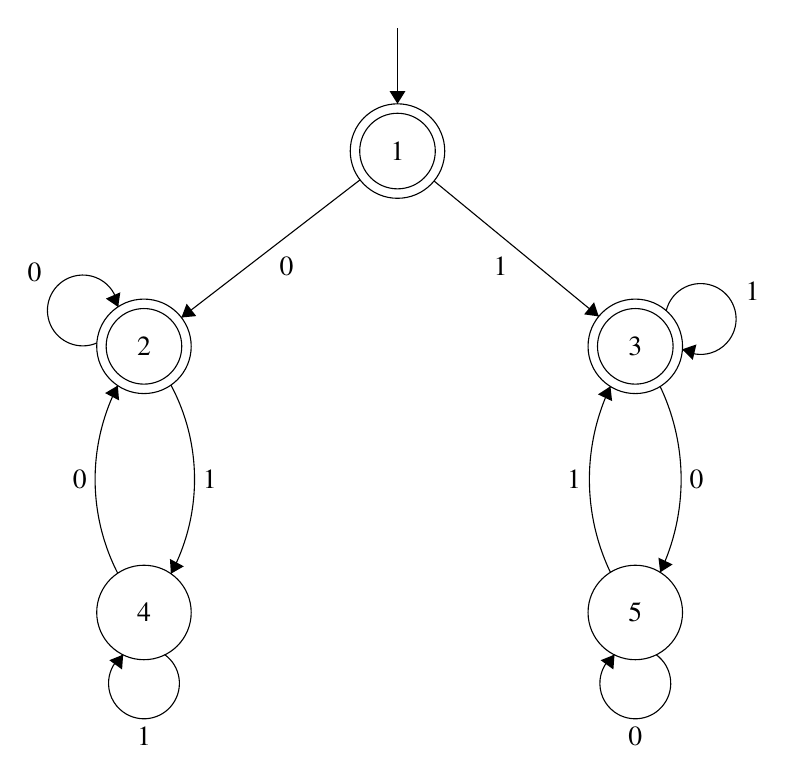
\begin{tikzpicture}[scale=0.2]
\tikzstyle{every node}+=[inner sep=0pt]
\draw [black] (39.8,-11) circle (3);
\draw (39.8,-11) node {$1$};
\draw [black] (39.8,-11) circle (2.4);
\draw [black] (23.7,-23.4) circle (3);
\draw (23.7,-23.4) node {$2$};
\draw [black] (23.7,-23.4) circle (2.4);
\draw [black] (54.9,-23.4) circle (3);
\draw (54.9,-23.4) node {$3$};
\draw [black] (54.9,-23.4) circle (2.4);
\draw [black] (23.7,-40.3) circle (3);
\draw (23.7,-40.3) node {$4$};
\draw [black] (54.9,-40.3) circle (3);
\draw (54.9,-40.3) node {$5$};
\draw [black] (37.42,-12.83) -- (26.08,-21.57);
\fill [black] (26.08,-21.57) -- (27.02,-21.48) -- (26.41,-20.69);
\draw (32.76,-17.7) node [below] {$0$};
\draw [black] (42.12,-12.9) -- (52.58,-21.5);
\fill [black] (52.58,-21.5) -- (52.28,-20.6) -- (51.65,-21.37);
\draw (46.34,-17.69) node [below] {$1$};
\draw [black] (25.411,-25.856) arc (28.11238:-28.11238:12.721);
\fill [black] (25.41,-37.84) -- (26.23,-37.37) -- (25.35,-36.9);
\draw (27.41,-31.85) node [right] {$1$};
\draw [black] (22.037,-37.811) arc (-152.84139:-207.15861:13.059);
\fill [black] (22.04,-25.89) -- (21.23,-26.37) -- (22.12,-26.83);
\draw (20.1,-31.85) node [left] {$0$};
\draw [black] (56.476,-25.946) arc (25.48915:-25.48915:13.72);
\fill [black] (56.48,-37.75) -- (57.27,-37.25) -- (56.37,-36.82);
\draw (58.31,-31.85) node [right] {$0$};
\draw [black] (53.322,-37.755) arc (-154.47246:-205.52754:13.703);
\fill [black] (53.32,-25.94) -- (52.53,-26.45) -- (53.43,-26.88);
\draw (51.48,-31.85) node [left] {$1$};
\draw [black] (39.8,-3.2) -- (39.8,-8);
\fill [black] (39.8,-8) -- (40.3,-7.2) -- (39.3,-7.2);
\draw [black] (56.223,-42.98) arc (54:-234:2.25);
\draw (54.9,-47.55) node [below] {$0$};
\fill [black] (53.58,-42.98) -- (52.7,-43.33) -- (53.51,-43.92);
\draw [black] (25.023,-42.98) arc (54:-234:2.25);
\draw (23.7,-47.55) node [below] {$1$};
\fill [black] (22.38,-42.98) -- (21.5,-43.33) -- (22.31,-43.92);
\draw [black] (20.72,-23.183) arc (293.5717:5.5717:2.25);
\draw (17.23,-18.73) node [left] {$0$};
\fill [black] (22.06,-20.9) -- (22.2,-19.97) -- (21.28,-20.37);
\draw [black] (56.862,-21.146) arc (166.68812:-121.31188:2.25);
\draw (61.87,-19.87) node [right] {$1$};
\fill [black] (57.88,-23.59) -- (58.55,-24.26) -- (58.78,-23.28);
\end{tikzpicture}
\end{center}

\end{enumerate}

\end{document}









